\chapter{Introducción}
\label{cap:capitulo1}
\setcounter{page}{1}

\begin{flushright}
	\begin{minipage}[]{10cm}
		\emph{Quizás algún fragmento de libro inspirador...}\\
	\end{minipage}\\

	Autor, \textit{Título}\\
\end{flushright}

\vspace{1cm}

En la actualidad los vehículos autónomos están en auge, cada vez tenemos más ejemplos de tareas típicamente realizadas por humanos que ya, es posible realizar sin un humano al mando. La conducción autónoma tiene el potencial para cambiar la forma en que nos movemos, aportando seguridad y comfort, si bien es cierto que aún no vemos vehículos circulando sin conductor, mucha de la tecnología necesaria para hacerlo ya está presente en los vehículos actuales. La conducción autónoma va mucho más allá de, únicamente los vehículos que transitan las ciudades, es aplicable a muchos otros ámbitos, por ejemplo entornos industriales, de inspección o incluso de exploración donde el vehículo se enfrenta a situaciones impredecibles y ante las que debe saber reaccionar correctamente.\\

\section{Coches autónomos}
\label{sec:cochesautonomos} % etiqueta para luego referenciar esta sección
Cuando se nos viene a la cabeza el concepto de vehículo autónomo, se suele relacionar con coches autónomos, es decir, los vehículos que circulan a diario por las ciudades; coches, autobuses, furgonetas pero sin una persona al volante. Todavía no está presente en las ciudades pero en un corto plazo de tiempo lo estará, el principal inconveniente actual es la regulación, a diferencia de, por ejemplo, el entorno de la aviación, donde desde hace décadas el control de la aeronave es autómatico a excepción de tareas como el despegue, el aterrizaje o situaciones de emergencia.\\

Actualmente coches de última generación como \textit{Tesla}, ya incorporan un grado de autonomía elevado en determinadas situaciones, pero siempre con un conductor al volante que debe permanecer atento para poder reaccionar.\\

\begin{figure} [h!]
	\begin{center}
		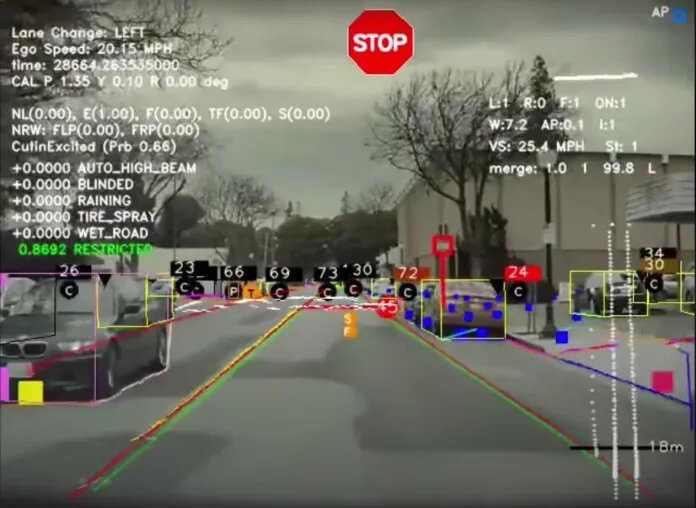
\includegraphics[width=12cm]{figs/tesla_object_detection}
	\end{center}
	\caption{\textit{Tesla AutoPilot}.}
	\label{fig:tesla_object_detection}
\end{figure}\

Niveles de autonomía \textit{SAE J3016}:

\begin{enumerate}
	\item Sin automatización
	\item Asistencia a la conducción
	\item Automatización parcial
	\item Automatización condicionada
	\item Automatización elevada
	\item Automatización completa
\end{enumerate}\

\begin{figure} [h!]
	\begin{center}
		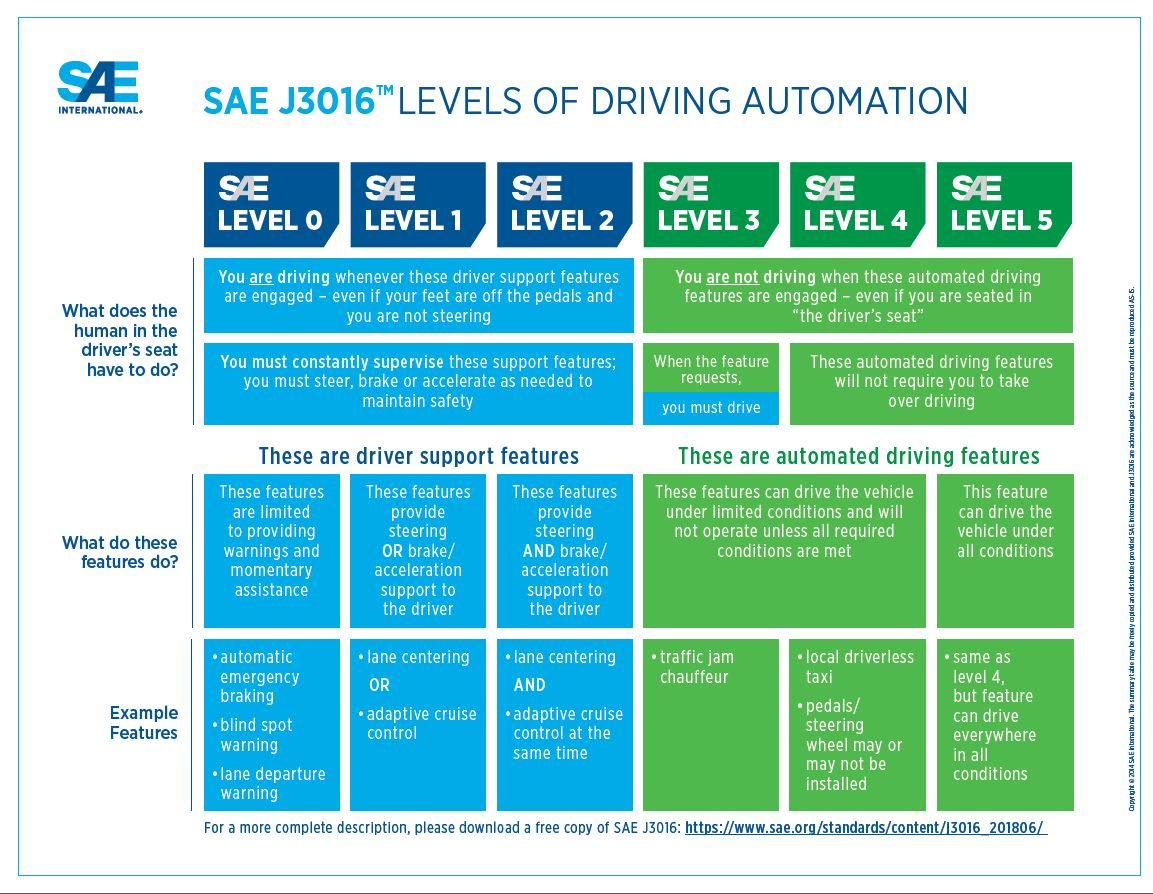
\includegraphics[width=12cm]{figs/SAEJ3016}
	\end{center}
	\caption{Niveles de autonomía \textit{SAE J3016}.}
	\label{fig:SAEJ3016}
\end{figure}\

\section{AMRs}
\label{sec:amr} % etiqueta para luego referenciar esta sección
Los  \textit{AMRs} son robots móviles autónomos, capaces de navegar por entornos dinámicos, conviviendo con humanos a su alrededor y sabiendo sobreponerse a situaciones para las que no habían sido programados explícitamente. Son los sucesores de los  \textit{AGVs}, vehículos guiados automatizados, este tipo de vehículos requieren una cierta infraestructura dependiendo del tipo de guiado, ya sea filoguiados, a través de pintura o a través de cualquier otra técnica que haga que ese vehículo sólo pueda funcionar cuando se sabe la infraestructura previa que estará presente en el entorno de trabajo.\\

Además, presentan muchas dificultades para relacionarse con obstáculos o humanos, donde ante un cambio pequeño del entorno, el robot se detendrá por seguridad. A diferencia de estos, los  \textit{AMRs}, son capaces de realizar multitud de tareas en entornos donde la infraestructura necesaria es casi nula, quizá tengan una serie de requisitos en cuanto a conectividad, pero con esa excepción, son robots que pueden ser diseñados para navegar por cualquier tipo de ambiente.\\

Un ejemplo muy representativo de  \textit{AMRs}, es \textit{Kiva Systems}, empresa comprada por \textit{Amazon} para automatizar sus almacenes en tareas de logística a nivel interno, maximizando la producción y el almacenamiento, tanto en profundidad como en altura y minimizando el coste en personal.\\

\begin{figure} [h!]
	\begin{center}
		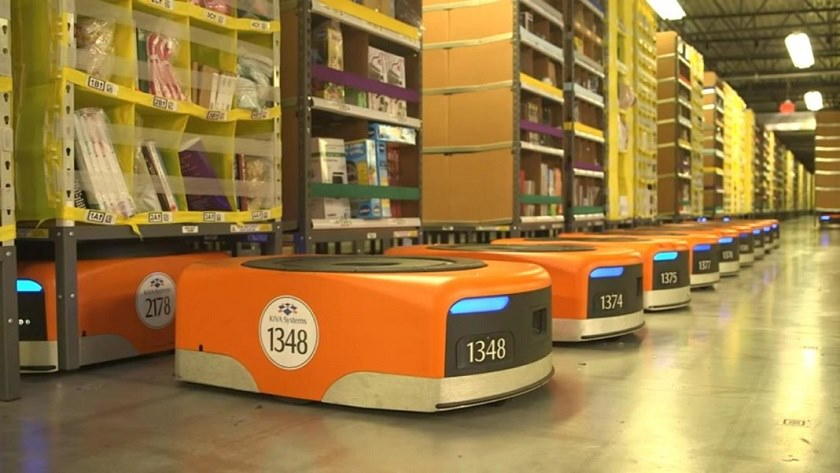
\includegraphics[width=8cm]{figs/kiva_systems}
	\end{center}
	\caption{\textit{AMRs Kiva Systems} en almacenes de \textit{Amazon}.}
	\label{fig:kiva_systems}
\end{figure}\

\section{Visión como sensor principal}
\label{sec:vision}
Gracias a un sensor como la cámara podemos obtener una información muy completa del entorno que rodea al robot y con ello poder actuar en consecuencia. La cámara se presenta como el sensor más interesante que puede equipar un robot, cuentan con un tamaño y peso muy reducido, como es el caso de la \ref{fig:picamera}, además de un coste muy reducido. Sin embargo, presenta algunas dificultades cuando nos disponemos a tratar la imagen recibida; en cuanto a potencia del dispositivo, para procesar una imagen, y dependiendo de su resolución, es necesario un mínimo de requerimientos técnicos a nivel de \textit{hardware}, para poder conseguir un procesamiento con un nivel adecuado de \textit{fps}, por otra parte, la imagen recibida deberá haber sido captada en un entorno con buenas condiciones lumínicas. Para ello existen diferentes tipos de sensores \textit{EO/IR}, como por ejemplo, cámaras de visión noctura, donde el espectro utilizado es \textit{FIR}, con ello se consigue resaltar en la imagen lo que realmente es necesario,

\begin{figure} [h!]
	\begin{center}
		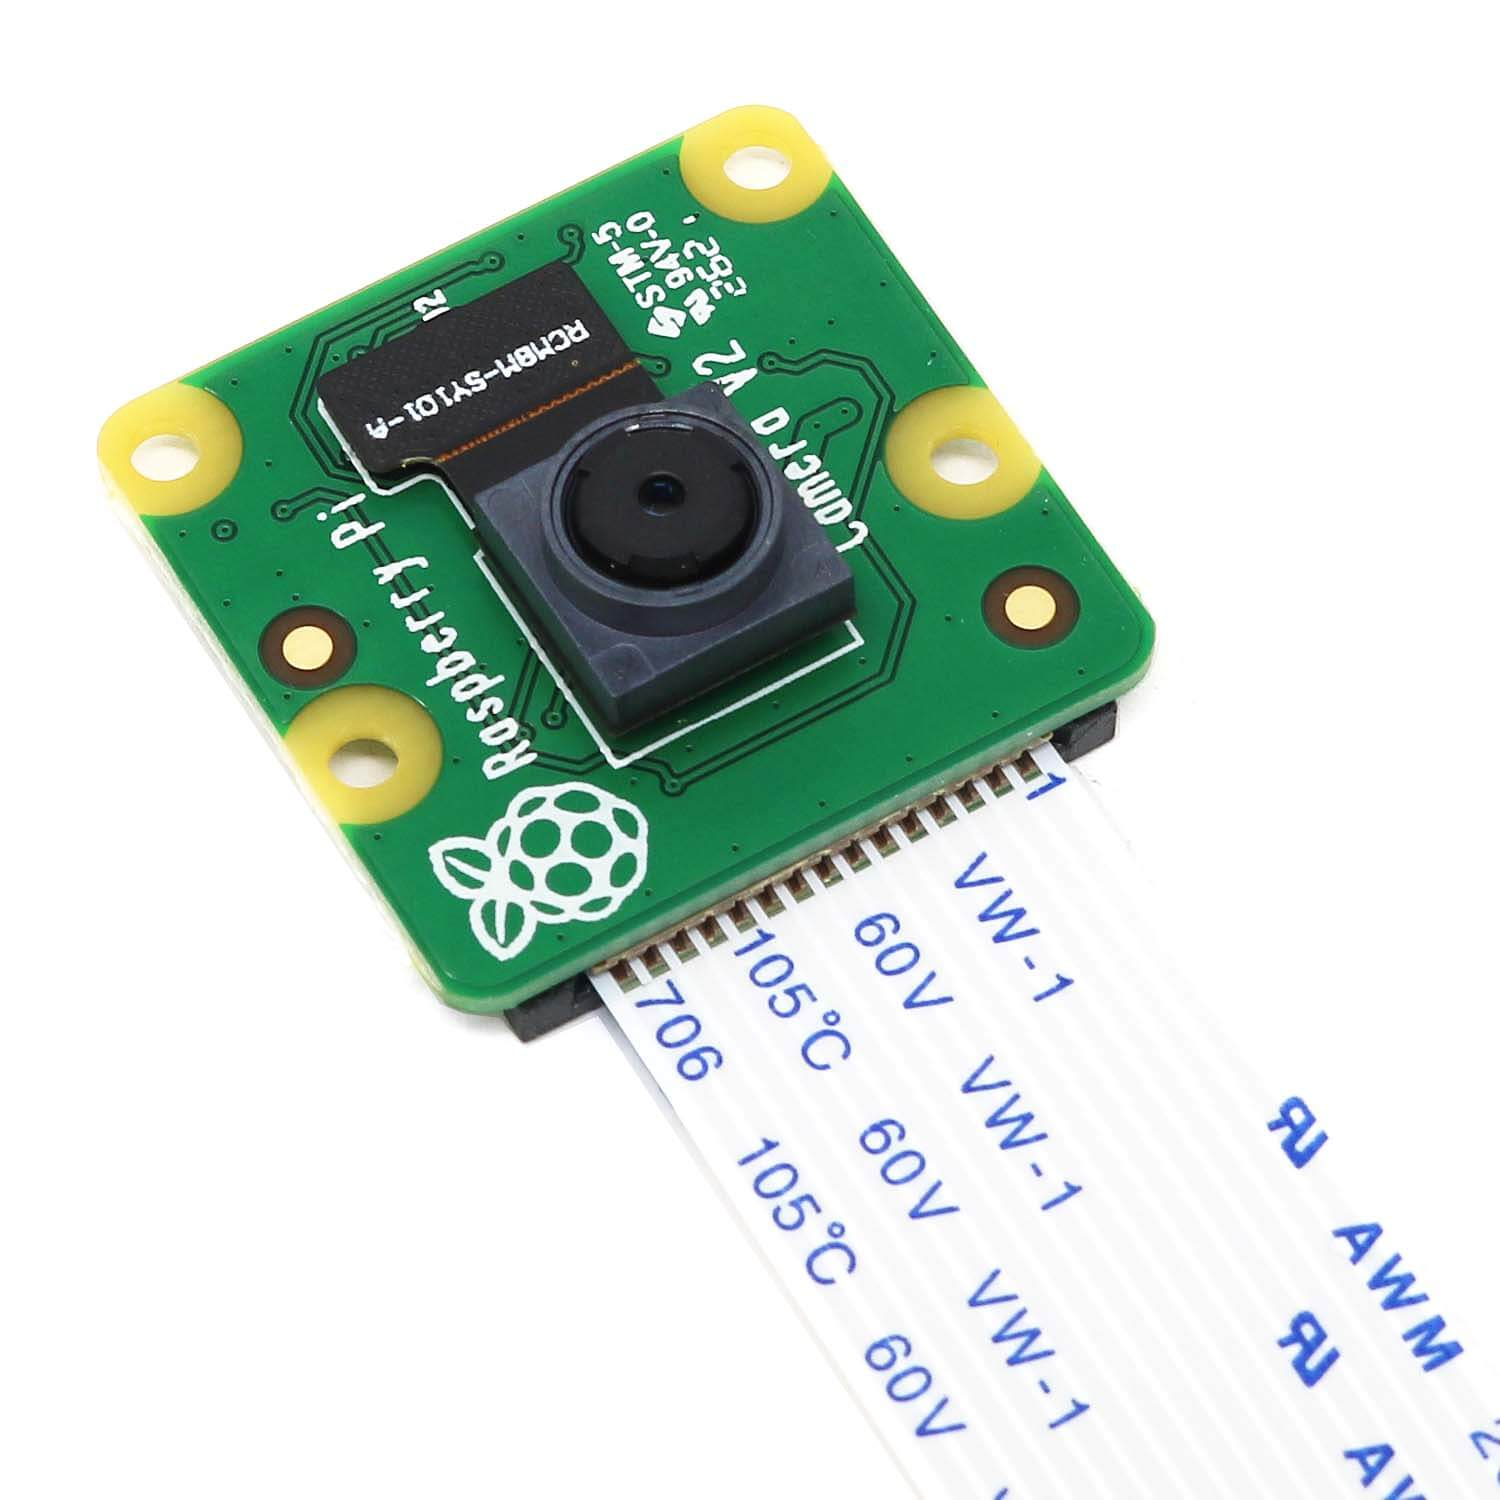
\includegraphics[width=4cm]{figs/picamera}
	\end{center}
	\caption{\textit{PiCamera} usada en la placa \textit{Raspberry Pi}.}
	\label{fig:picamera}
\end{figure}\

Un ejemplo es \textit{BMW's FIR-based Autoliv Night Vision System}, trabaja con imagenes de \textit{320x240} y cuenta con un rango de \textit{300 metros}.\\

\begin{figure} [h!]
	\begin{center}
		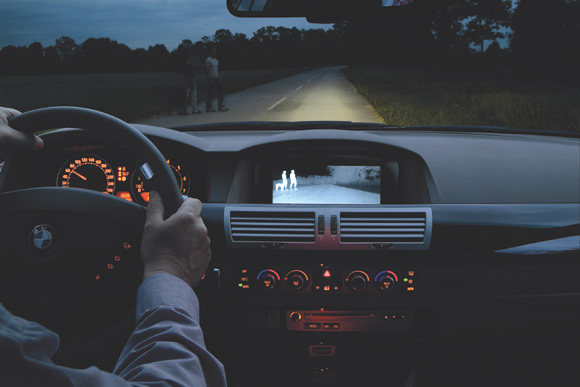
\includegraphics[width=8cm]{figs/night_vision}
	\end{center}
	\caption{\textit{BMW's FIR-based Autoliv Night Vision System}.}
	\label{fig:nightvision}
\end{figure}\

Cuando se realiza el procesamiento de una imagen, es interesante conocer la distancia, por ejemplo, a la que se encuentra un objeto en concreto, para ello existen soluciones para poder conocer dicha información con una cámara tradicional, es el caso de \textit{cite Open Vision System for Low-Cost Robotics Education} o \textit{OpenCV distance}, sin embargo, estos algoritmos se basan en la suposición de que todos los objetos se encuentras situados en un plano imaginario situado en el suelo. Para eliminar esta restricción, y poder conocer distancias de objetos que no se encuentran situados en el suelo, surgen las \textit{cámaras RGBD}, en la que cada píxel de la imagen proporciona además del color RGB, una tercera componente llamada \textit{depth}. Una de las primeras \textit{cámaras RGBD} comerciales es la \textit{Kinect} desarrollada por \textit{Microsoft} para su consola \textit{Xbox 360}.\\

\begin{figure} [h!]
	\begin{center}
		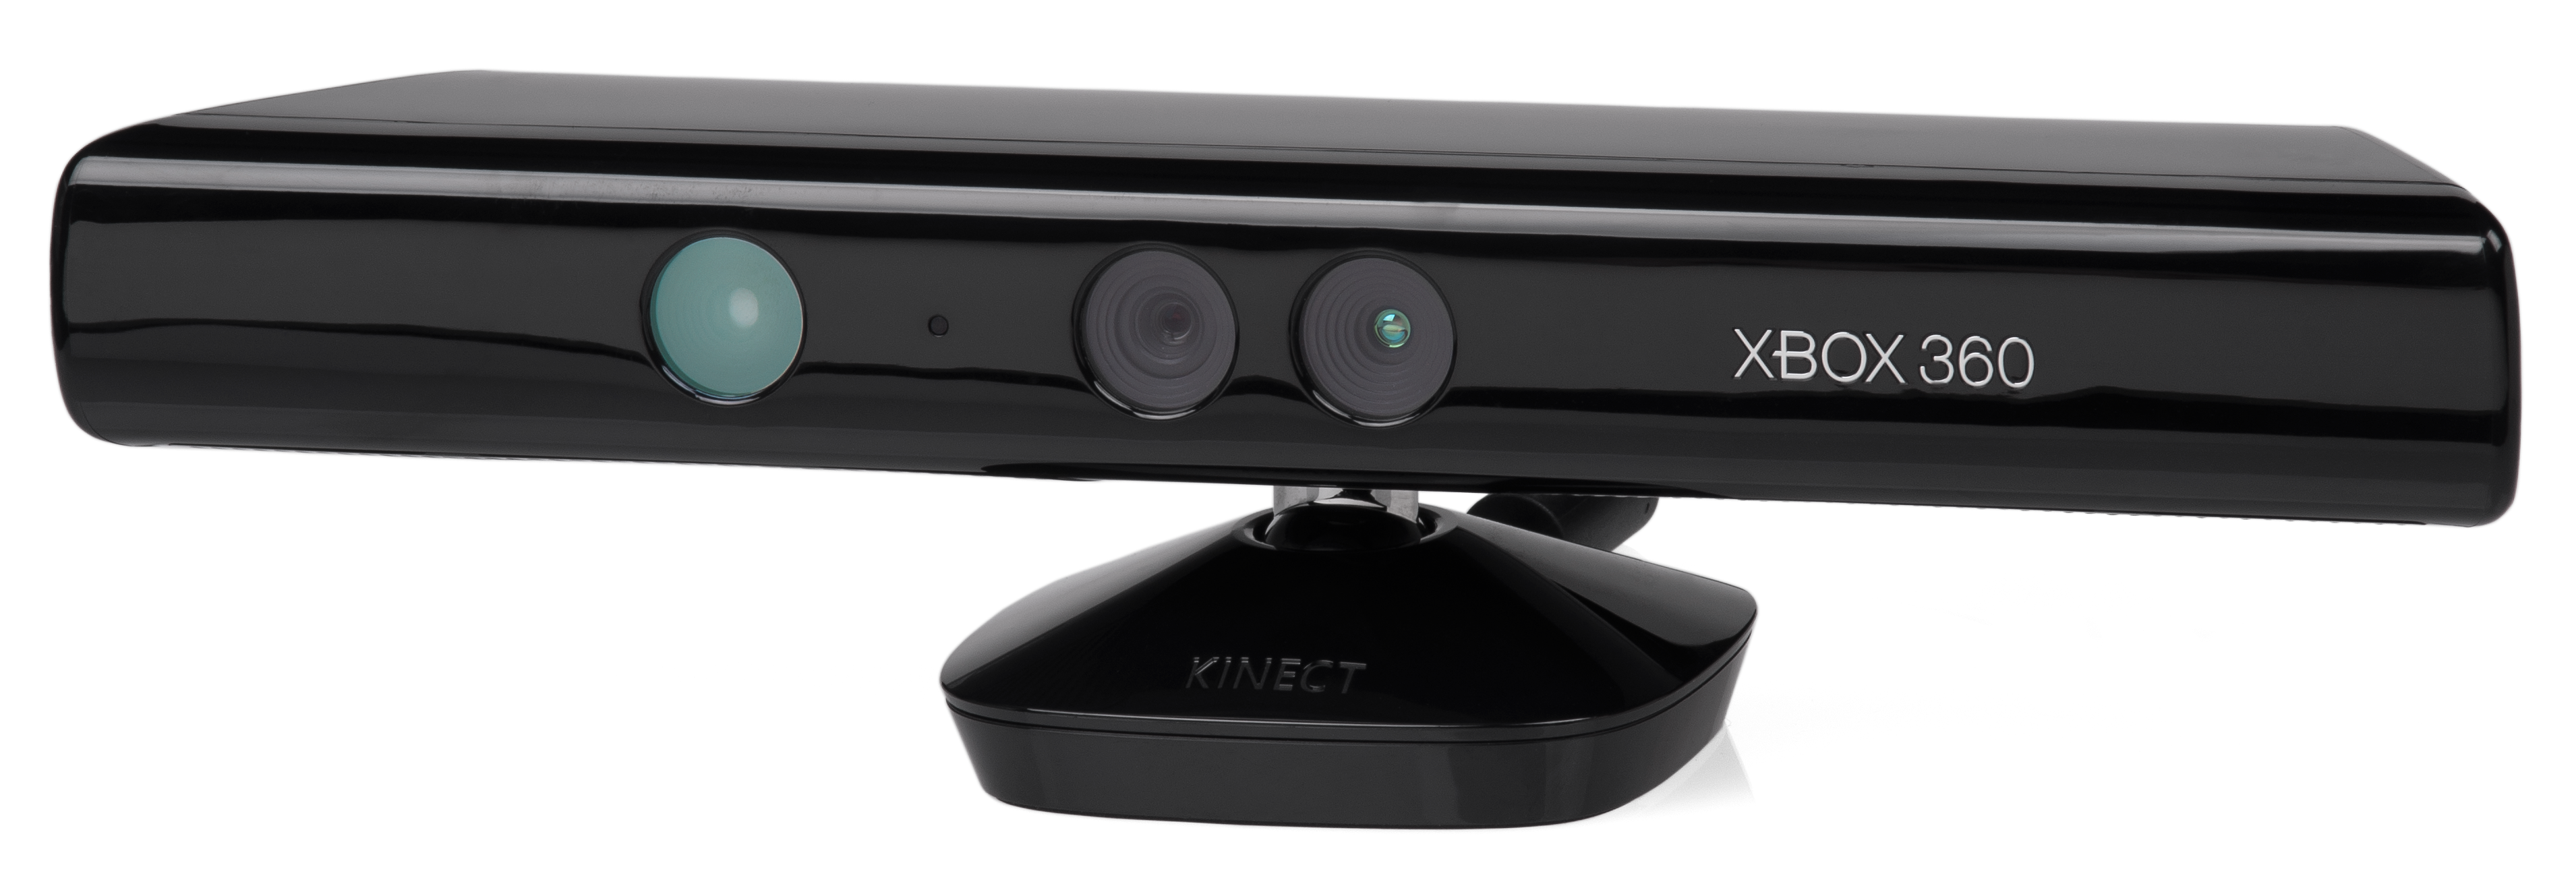
\includegraphics[width=8cm]{figs/kinect}
	\end{center}
	\caption{\textit{Kinect} desarrollada por \textit{Microsoft}.}
	\label{fig:kinect}
\end{figure}\

\begin{figure} [h!]
	\begin{center}
		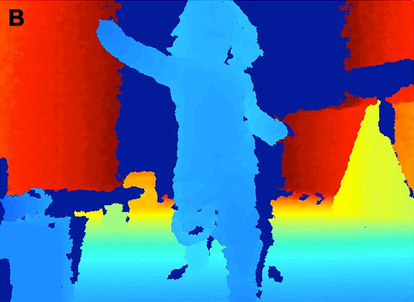
\includegraphics[width=8cm]{figs/depth}
	\end{center}
	\caption{Imagen de profundidad \textit{Kinect}.}
	\label{fig:depth}
\end{figure}\

La visión artificial ofrece multitud de posibilidades, no solo en robótica, tiene una gran de aplicaciones en campos tan dispares como la medicina, la realidad aumentada, el procesamiento de señales o la agricultura.\\

\section{Arquitectura}
\label{sec:arquitectura}
La decisión de qué arquitectura utilizar en un robot es determinante. Es necesario evaluar multitud de factores; consumo de energía, potencia requerida, tamaño y peso, sistema operativo a utilizar, posibilidad de recibir respuesta en \textit{real time}, precio etc...

Existen multitud de arquitecturas utilizadas en proyectos robóticos \textit{x86}, \textit{x86-64}, \textit{ARMv6}, \textit{ARMv7} o \textit{AArch64}. Pero, actualmente hay dos arquitecturas predominantes \textit{x86-64} y \textit{AArch64}, ambas de \textit{64 bits}, ya que los 32 bits han quedado desfasados para la gran mayoría de aplicaciones, además de que, los nuevos sistemas operativos comienzan a no soportarlos. \cite{canonical32bits}

Estas dos arquitecturas tienen grandes diferencias en cuanto al diseño de los procesadores y las instrucciones que utilizan:
\begin{itemize}
	\item Reduced Instruction Set Computer (\textit{RISC})
	\item Complex Instruction Set Computer (\textit{CISC})
\end{itemize}\

El conjunto de instrucciones utilizado por \textit{AArch64} es \textit{CISC}, este conjunto se compone de gran cantidad de instrucciones y muchas de ellas complejas para realizar tareas que, el conjunto \textit{RISC}, puede realizar con varias instrucciones. Este último conjunto es utilizado por la arquitectura \textit{x86-64}.\\

Ejemplos representativos de \textit{AArch64}:
\begin{figure} [h!]
	\begin{center}
		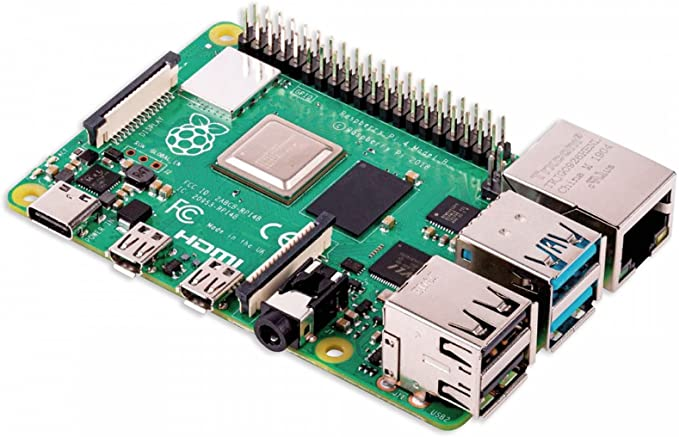
\includegraphics[width=6cm]{figs/raspberrypi}
	\end{center}
	\caption{\textit{Raspberry Pi 4}.}
	\label{fig:raspberrypi}
\end{figure}\

\begin{figure} [h!]
	\begin{center}
		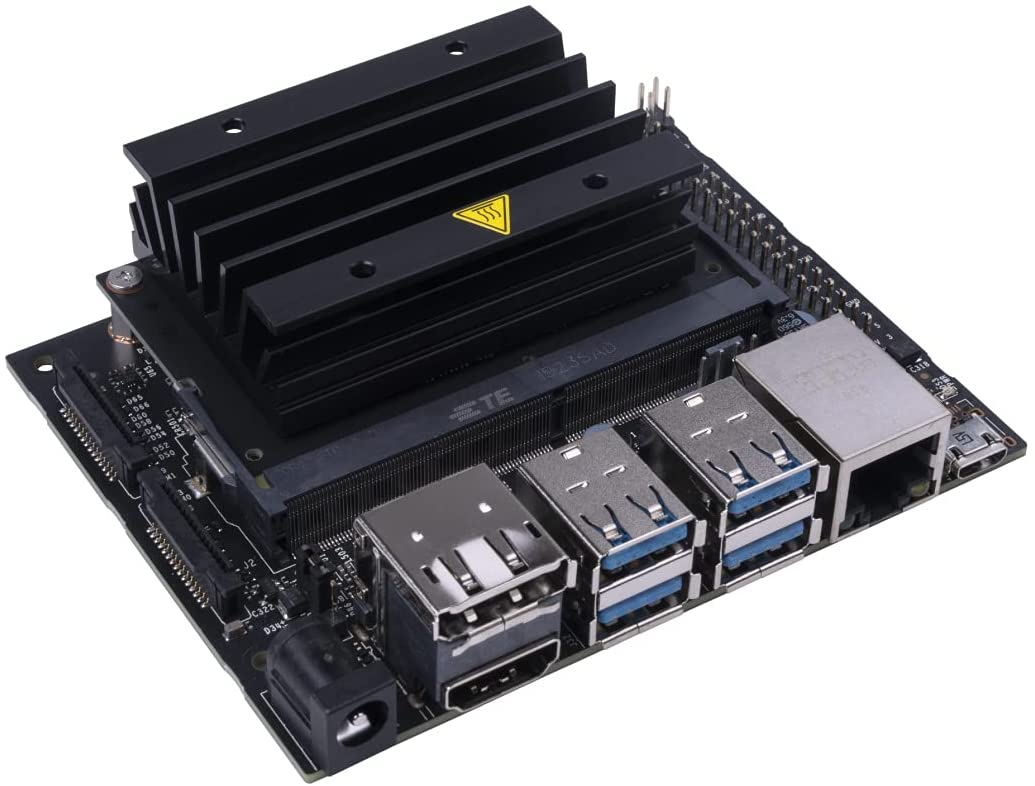
\includegraphics[width=6cm]{figs/jetson_nano}
	\end{center}
	\caption{\textit{Jetson Nano}.}
	\label{fig:jetsonnano}
\end{figure}\

Ejemplos representativos de \textit{x86-64}:

\begin{figure} [h!]
	\begin{center}
		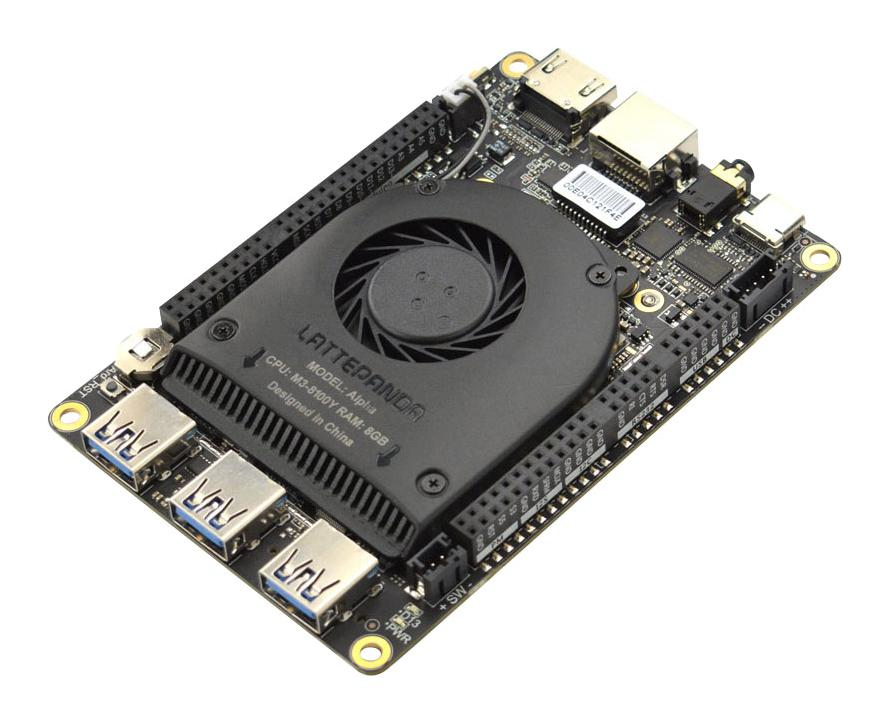
\includegraphics[width=6cm]{figs/lattepanda}
	\end{center}
	\caption{\textit{LattePanda Alpha 864s}.}
	\label{fig:lattepanda}
\end{figure}\

\begin{figure} [h!]
	\begin{center}
		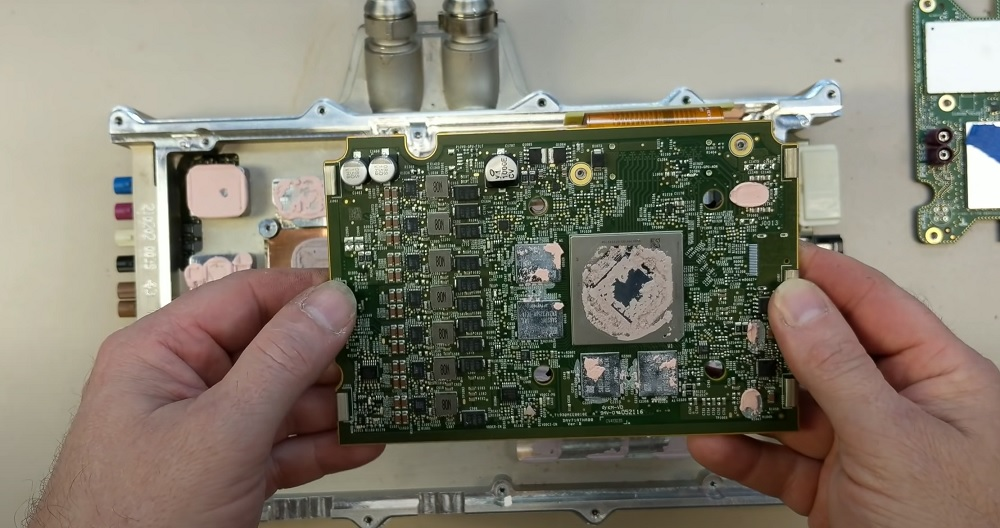
\includegraphics[width=6cm]{figs/tesla_zen_rdna2}
	\end{center}
	\caption{\textit{AMD Zen} como CPU y \textit{Navi 23} como GPU, usado en Tesla Model S.}
	\label{fig:teslazenrdna2}
\end{figure}\

\section{Deep Learning}
\label{sec:deeplearning}
El \textit{Deep Learning} se basan en redes neuronales que parten del \textit{Machine Learning}, que a su vez surge de la \textit{Inteligencia Artificial} (\textit{IA}). Sus inicios se remontan al año 1979 cuando \textit{Kunihiko Fukushima} desarrolló una red neuronal de entre 5 y 6 capas llamada \textit{neocognitrón}, con el objetivo de reconocer carácteres japoneses 

\begin{figure} [h!]
	\begin{center}
		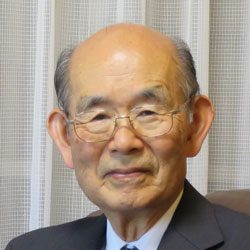
\includegraphics[width=4cm]{figs/kuni}
	\end{center}
	\caption{\textit{Kunihiko Fukushima}, buscar imagen reconocimiento carácteres japoneses .}
	\label{fig:kuni}
\end{figure}\


Este tipo de redes neuronales tienen multitud de aplicaciones, pero principalmente todas comparten grandes cantidades de datos, en cualquier formato; vídeo, imagen, sonido. Algunas de ellas son; clasificación de objetos, \textit{Natural language processing} (\textit{NLP}), Big Data, anaĺisis médico, conversiñón de imágenes en blanco y negro a color etc...

\subsection{\textit{Convolutional neural network} (\textit{CNN})}
\label{sec:cnn}

$1.5Kg$ 1.500\euro.

\subsection{\textit{ResNet}}
\label{sec:resnet}

\subsection{YOLO}
\label{sec:yolo}

\textit{YOLO}
\begin{figure} [h!]
	\begin{center}
		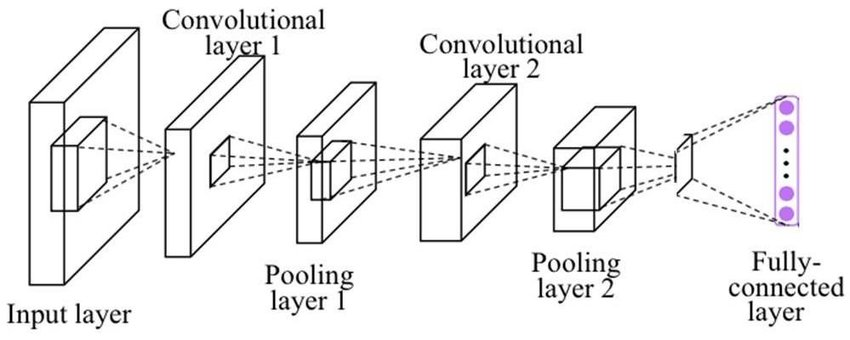
\includegraphics[width=8cm]{figs/yolo}
	\end{center}
	\caption{\textit{YOLO}.}
	\label{fig:yolo}
\end{figure}\

\paragraph{Referencias bibliográficas}
\label{sec:referencias}

Citas libros, artículos, URLs, tesis, congresos

Las referencias \texttt{bibliografia.bib}. El contenido de estas referencias está en formato \texttt{BibTex}. Obtener de \texttt{Google Scholar} u otros repositorios de recursos científicos.

\

\

\

En los siguientes capítulos trataremos los objetivos a cumplir ...
Números páginas
Barra baja, != dolar
Imágenes horizontal
Siglas en inglés?
